% Material moved out of the paper in the focused rewrite of 2026-11-19
% (from simtix_tvlsi_long_2026-11-19.tex), included by simtix_tvlsi_supp.tex.

\section{Benchmark Rules and Changes}\label{sup:bench}
Each Rodinia benchmark is defined by Rodinia's computation on Rodinia's data: the
sequence of FP32 operations that produces one output, each rounded once, with a fused
multiply-add where the sum is fused. The input files are Rodinia's own. Work that
Rodinia performs on the CPU (the control of the bfs levels, the selection of the nearest
records in nn, the center update of kmeans and the back substitution of gaussian) runs
on the A53 for every machine and is not timed. For SIMTiX and Vortex, the A53's timer
measures from the first launch to the end of the last, including the host's work
between launches; for CVA6 and Ara, the cycle counter of CVA6 measures the kernel,
whose loop over iterations runs on CVA6 itself.

Three choices depart from Rodinia's default runs. All machines compute in FP32.
backprop uses 2$^{19}$ inputs rather than 2$^{21}$, whose two 256~MiB weight arrays do
not fit the memory region of the Ara host. gaussian uses the matrix that Rodinia
generates rather than its matrix file: Rodinia eliminates without pivoting, and on the
random matrix of the file the entries grow to $5.3\times10^{4}$, so that a change of one
ulp in 8.7\% of the quotients changes rows of the result by up to 6.3 times their
largest entry. This matters because the divide and square-root unit of CVA6, which Ara
shares, is not correctly rounded: on 4,096 random operands, 8.7\% of its quotients and
6.9\% of its square roots differ from the correctly rounded value by one ulp. Finally,
Ara computes gaussian's multipliers (Rodinia's Fan1 kernel, one division per row) on
CVA6, because its vector form returned wrong values, or deadlocked, when it ran after
nn; the elimination itself (Fan2) runs on Ara.

RiVEC computes in FP64; all machines here compute in FP32, the precision of SIMTiX and
Vortex. Each RiVEC application is defined by RiVEC's vector code read per element, with
RiVEC's fused multiply-adds and its polynomial exponential and logarithm; sums over many
elements (a row of spmv, the force on a particle in lavaMD) are defined in serial
order. SIMTiX, Vortex and CVA6 then produce the A53 reference bit for bit, and so does
Ara except in spmv and lavaMD, where its code keeps one partial sum per vector element
and reduces them at the end. blackscholes divides three times and takes one square root
per option; with the divide and square-root unit of CVA6, CVA6 and Ara give identical
prices that differ from the reference by up to $5.7\times10^{-4}$ of $|p|+0.01$. A model
of RiVEC's computation in which each quotient and square root is one ulp off at the
measured rates of 8.7\% and 6.9\% gives the same bound over 200 random trials on the
same options; the limit is $10^{-3}$.

RiVEC's code was changed in four places. Two are errors in RiVEC. Its blackscholes
negates the cumulative normal of the negative arguments with a masked subtract in the
mask-agnostic form, which allows an RVV~1.0 implementation to overwrite the unselected
elements; under QEMU, 46,277 of the 65,536 prices are wrong. We select the two results
with a merge instead. RiVEC's spmv builds the matrix from the file's column-major
entries with one-based indices and reads one element past the end of $x$; we use
zero-based indices, which computes $y=A^{\mathsf T}x$ for RiVEC's matrix. The other two
changes avoid faults of Ara. Ara reloads a vector register spilled to the stack with
wrong values, and GCC spills one in blackscholes, so RiVEC's code is compiled with
clang, which does not. Ara's jacobi-2d computed wrong last elements of some rows,
differently from run to run, when it ran after another kernel, while it reused vector
registers from one row to the next; it now loads the three rows for every output row,
which costs about 46\% more cycles in a reduced run.

\section{FP16 Arithmetic}\label{sup:fp16}
The FPU has five pipeline stages, and its 48-bit significand product is formed on a
$24\times24$ cascade of DSP blocks. FP16 operations widen their operands to FP32, use
the FP32 datapath and round the result to FP16, so an FP16 result is rounded twice. Let
$\circ_p$ denote rounding to nearest even and $\square_p$ rounding to odd, at $p$ bits
of significand: 24 for FP32, 11 for FP16.

\newtheorem{sproposition}{Proposition}
\renewcommand{\thesproposition}{S\arabic{sproposition}}
\begin{sproposition}
Let $x$ be the exact sum, difference, product, quotient or square root of FP16
operands, and $y=ab+c$ the exact result of an FMA of FP16 operands, with results in the
normal range of FP16. Then $\circ_{11}(\circ_{24}(x))=\circ_{11}(x)$ and
$\circ_{11}(\square_{24}(y))=\circ_{11}(y)$.
\end{sproposition}
\begin{IEEEproof}
For the five basic operations, double rounding to nearest is innocuous when the
intermediate precision $p$ and the target precision $q$ satisfy
$p\ge2q+2$~\cite{figueroa}; here $24=2\cdot11+2$. The exact result of an FMA is not the
result of such an operation on $q$-bit operands, so that bound does not apply. For any
real $y$, rounding to odd at $p\ge q+2$ bits followed by rounding to nearest at $q$
bits equals rounding to nearest at $q$ bits~\cite{boldo}, and $24\ge13$. FP32 contains
the exponent range of FP16, so neither rounding is affected by underflow or overflow
within the normal range.
\end{IEEEproof}

The FPU therefore rounds an FMA with an FP16 destination to odd at FP32 precision, and
its FP16 results in the default rounding mode are correctly rounded; the directed modes
are covered by the test vectors. We checked the units bit-exactly against an IEEE-754
reference~\cite{ieee754} on 116,089 arithmetic and 100,884 conversion vectors that
cover every rounding mode.

\section{Suite~2 and the Synchronization Kernels}\label{sup:suite2}
The board runs of Section~\ref{P-sec:lanes16} include a second suite of ten kernels,
\emph{suite~2}, drawn from five benchmark suites: pathfinder, hotspot and backprop from
Rodinia, Black-Scholes from RiVEC, PageRank and connected components from
GAP~\cite{gap}, the radix sort of SHOC~\cite{shoc}, and ATAX, BiCG and Jacobi-2D from
PolyBench~\cite{polybench}. Suite~2 follows the rules of the applications: each kernel
is defined by the sequence of FP32 operations of one output, SIMTiX runs hand-written
assembly, the A53 runs one C version and checks every output, and every kernel runs at
two input sizes. CVA6 and Ara also run suite~2 (Vortex has no ports of it); at the
larger input, the eight-lane SIMTiX is $14.6\times$ and $3.4\times$ faster than CVA6 and
Ara and the 16-lane SIMTiX $17.0\times$ and $4.0\times$ (geometric means), and Ara is
faster on Black-Scholes, whose results on CVA6 and Ara differ from SIMTiX's in the last
bits through their divider's rounding. FGPU also runs suite~2: the eight-lane SIMTiX is
$4.16\times$ faster at the larger input (geometric mean), from $2.05\times$ on hotspot to
$19.7\times$ on ATAX and BiCG, whose row-wise product gives each work-item of a wavefront
its own cache line at every step while FGPU fills two lines at a time, and
FGPU is faster on Black-Scholes (0.23 of SIMTiX's time), which divides.

\begin{figure*}[t]
\centering
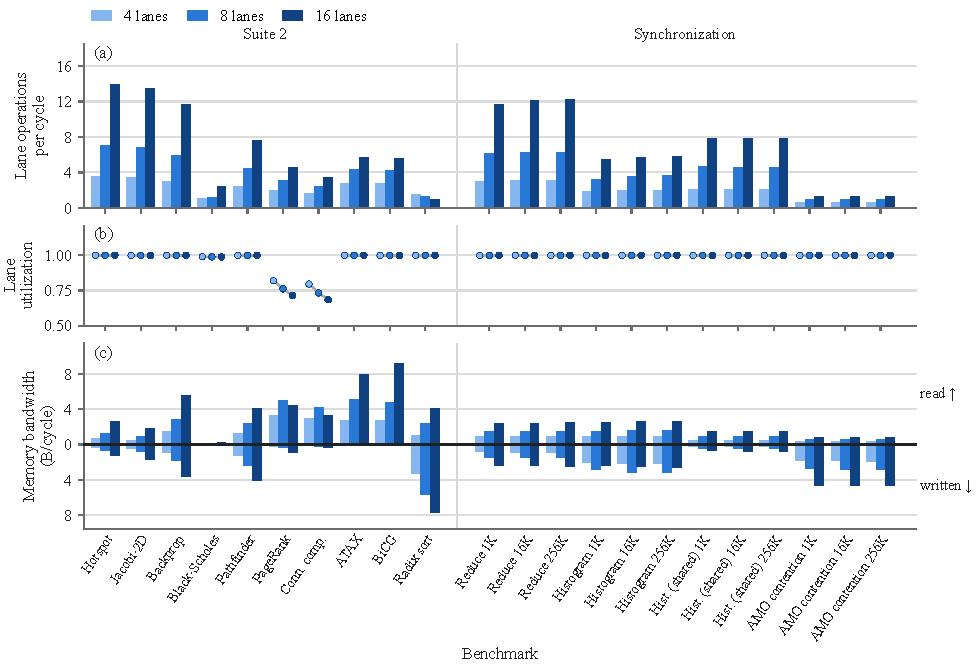
\includegraphics[width=\textwidth]{lanes_metrics_supp.pdf}
\caption{Throughput, lane utilization and memory bandwidth of suite~2 and the
synchronization kernels at 4, 8 and 16 lanes in simulation. (a) Lane operations per
cycle. (b) Lane utilization. (c) Bytes read (up) and written (down) per cycle.}
\label{fig:lanes_s2sync}
\end{figure*}

Fig.~\ref{fig:lanes_s2sync} completes the lane-scaling study of
Section~\ref{P-sec:evallanes} of the paper; the synchronization kernels run at 1K, 16K
and 256K threads. At four, eight and 16 lanes, the geometric-mean throughput is 2.24,
3.49 and 5.33 lane operations per cycle for suite~2, with a lane utilization of 0.96,
0.94 and 0.93, and 1.68, 3.09 and 5.12 for the synchronization kernels, whose lanes
never diverge. The utilization of PageRank and connected components falls from 0.82
and 0.80 at four lanes to 0.71 and 0.69 at 16, for the reason given for BFS in the
paper. Black-Scholes is flat from four to eight
lanes and $2\times$ at 16 (one divide/square-root unit below 16 lanes). The block-shared
histogram gains $2.2\times$ from four to eight lanes: at four lanes its 32-thread blocks
take all eight warps, so each block barrier stalls the whole machine. Radix sort slows
as lanes are added ($0.90\times$ and $0.67\times$), because its scattered stores move
lines of one word per lane: its write traffic rises from 3.3 to 7.7 bytes per cycle
while its throughput falls. ATAX and BiCG read the most, 7.9 and 9.1 bytes per cycle at
16 lanes, of the 16 the port carries. At four lanes, the eight-thread groups of the AMO-contention
kernel span two warps whose order is not defined, so its check covers the results that
do not depend on that order: every \texttt{amoadd} sum and every \texttt{amomax}
maximum, which a lost update would change.

\section{Throughput Against the Peak}\label{sup:lanestp}
Tables~\ref{tab:lanes_tp} and~\ref{tab:lanes_cyc} give the useful throughput and the
cycles of 15 applications at 4, 8 and 16 lanes in simulation, with one 64~KiB L1 and one
divide/square-root unit at every lane count, eight warps, 16 MSHRs, 16 tags and an AXI4
memory model of 24 cycles, every output checked. The \emph{throughput} counts only the
useful operations: FP32 operations, with an FMA counted as two; INT8
multiply-accumulates for the CNN and the MLP; and lane operations, the issued warp
instructions times their active lanes, for the integer kernels. The \emph{ideality} is
the throughput divided by the peak, $2L$ FLOP, $4L$ MAC or $L$ lane operations per
cycle, and the speedup of a doubling is the ratio of the cycles before and after it. The compute kernels gain 1.93 to $2.05\times$ per doubling at constant IPC and
ideality; their ideality is set by the instructions that compute addresses and control
loops: 0.14 for GEMM against 0.47 for the register-blocked GEMM-RB. The gather kernels
gain 1.27 to $1.60\times$ per doubling, and their IPC falls, from 0.73 to 0.39 for
SpMV-Z.

\begin{table*}[t]
\caption{Throughput and Ideality at 4, 8 and 16 Lanes}
\label{tab:lanes_tp}
\centering\footnotesize
\setlength{\tabcolsep}{4.5pt}
\begin{tabular}{llrrrrrr}
\toprule
Kernel (board input) & Metric & \multicolumn{3}{c}{Throughput} & \multicolumn{3}{c}{Ideality}\\
\cmidrule(lr){3-5}\cmidrule(lr){6-8}
 & & 4 lanes & 8 lanes & 16 lanes & 4 & 8 & 16\\
\midrule
GEMM ($n=128$)             & FLOP/cycle    & 1.08 & 2.17 & 4.36           & 0.14 & 0.14 & 0.14\\
GEMM-RB ($n=128$)          & FLOP/cycle    & 3.80 & 7.63 & \textbf{14.86} & 0.47 & 0.48 & 0.46\\
Stencil ($128^2$)          & FLOP/cycle    & 0.61 & 1.22 & 2.40           & 0.08 & 0.08 & 0.08\\
Stencil-RB ($128^2$)       & FLOP/cycle    & 1.34 & 2.63 & 5.09           & 0.17 & 0.16 & 0.16\\
Embedding bag (256 bags)   & FLOP/cycle    & 0.43 & 0.88 & 1.76           & 0.05 & 0.05 & 0.05\\
SpMV (4096 rows)           & FLOP/cycle    & 0.31 & 0.49 & 0.69           & 0.04 & 0.03 & 0.02\\
SpMV-Z (4096 rows)         & FLOP/cycle    & 0.38 & 0.56 & 0.71           & 0.05 & 0.03 & 0.02\\
CNN, INT8 ($32^2$)         & MAC/cycle     & 3.36 & 6.74 & \textbf{13.46} & 0.21 & 0.21 & 0.21\\
MLP, INT8 (batch 16)       & MAC/cycle     & 1.36 & 2.71 & 5.31           & 0.08 & 0.08 & 0.08\\
k-means (16k points)       & lane-op/cycle & 3.40 & 6.77 & \textbf{13.43} & 0.85 & 0.85 & 0.84\\
k-means-U (16k points)     & lane-op/cycle & 3.41 & 6.67 & 12.31          & 0.85 & 0.83 & 0.77\\
BFS (16k vertices)         & lane-op/cycle & 1.59 & 2.36 & 3.41           & 0.40 & 0.30 & 0.21\\
Scan (64k elements)        & lane-op/cycle & 2.73 & 5.11 & 9.26           & 0.68 & 0.64 & 0.58\\
Segmented scan (64k)       & lane-op/cycle & 2.65 & 5.48 & 11.03          & 0.66 & 0.68 & 0.69\\
Hash join (16k probes)     & lane-op/cycle & 2.00 & 2.98 & 3.98           & 0.50 & 0.37 & 0.25\\
\bottomrule
\end{tabular}

\end{table*}

\begin{table*}[t]
\caption{Cycles, IPC and Speedup From Doubling the Lanes}
\label{tab:lanes_cyc}
\centering\footnotesize
\setlength{\tabcolsep}{4.5pt}
\begin{tabular}{lrrrrrrrr}
\toprule
Kernel & \multicolumn{3}{c}{Cycles} & \multicolumn{3}{c}{IPC} & \multicolumn{2}{c}{Speedup}\\
\cmidrule(lr){2-4}\cmidrule(lr){5-7}\cmidrule(lr){8-9}
 & 4 lanes & 8 lanes & 16 lanes & 4 & 8 & 16 & $4\to8$ & $8\to16$\\
\midrule
GEMM           & 3,880,530 & 1,933,322 & 962,975   & 0.97 & 0.97 & 0.98 & $2.01\times$ & $2.01\times$\\
GEMM-RB        & 1,104,255 & 549,599   & 282,239   & 0.94 & 0.94 & 0.91 & $2.01\times$ & $1.95\times$\\
Stencil        & 645,220   & 323,558   & 163,509   & 0.84 & 0.84 & 0.83 & $1.99\times$ & $1.98\times$\\
Stencil-RB     & 293,823   & 149,285   & 77,252    & 0.83 & 0.81 & 0.79 & $1.97\times$ & $1.93\times$\\
Embedding bag  & 306,918   & 149,493   & 74,476    & 0.77 & 0.79 & 0.79 & $2.05\times$ & $2.01\times$\\
CNN (INT8)     & 4,213,951 & 2,100,529 & 1,051,662 & 0.75 & 0.75 & 0.75 & $2.01\times$ & $2.00\times$\\
MLP (INT8)     & 2,778,021 & 1,388,607 & 709,769   & 0.70 & 0.70 & 0.68 & $2.00\times$ & $1.96\times$\\
k-means        & 1,683,383 & 844,828   & 425,681   & 0.85 & 0.85 & 0.84 & $1.99\times$ & $1.98\times$\\
k-means-U      & 1,049,558 & 536,692   & 290,751   & 0.85 & 0.83 & 0.77 & $1.96\times$ & $1.85\times$\\
Segmented scan & 511,400   & 282,781   & 158,199   & 0.66 & 0.69 & 0.69 & $1.81\times$ & $1.79\times$\\
Scan           & 1,436,259 & 813,498   & 483,430   & 0.72 & 0.68 & 0.61 & $1.77\times$ & $1.68\times$\\
SpMV           & 209,987   & 131,585   & 94,319    & 0.77 & 0.68 & 0.50 & $1.60\times$ & $1.40\times$\\
BFS            & 1,667,225 & 1,121,490 & 776,421   & 0.71 & 0.67 & 0.59 & $1.49\times$ & $1.44\times$\\
Hash join      & 270,265   & 181,411   & 135,937   & 0.71 & 0.66 & 0.54 & $1.49\times$ & $1.33\times$\\
SpMV-Z         & 170,211   & 116,877   & 91,978    & 0.73 & 0.58 & 0.39 & $1.46\times$ & $1.27\times$\\
\bottomrule
\end{tabular}

\end{table*}

\section{Simulated Applications and Timing Closure}\label{sup:sim}
\begin{table}[t]
\caption{Applications and Their Inputs}
\label{tab:apps}
\centering\footnotesize
\setlength{\tabcolsep}{2.6pt}
\begin{tabular}{llrrrrl}
\toprule
App. & Simulated input & Cycles & IPC & Util. & L1 hit & Board input\\
\midrule
GEMM    & $32^3$               & 45,902  & 0.69 & 100\% & 93\% & $256^3$\\
SpMV    & $512^2$, $\le$16/row & 26,295  & 0.43 & 59\%  & 88\% & $65{,}536^2$\\
Stencil & $32^2$, 2 sweeps     & 17,529  & 0.48 & 100\% & 88\% & $512^2$, 4\\
k-means & 1,024, $k=8$         & 36,935  & 0.66 & 100\% & 93\% & $2^{18}$, 16\\
BFS     & 1,024, degree 6      & 71,151  & 0.56 & 43\%  & 84\% & $2^{18}$, 8\\
Scan    & 2,048                & 34,468  & 0.50 & 95\%  & 73\% & $2^{20}$\\
MLP     & 784-128-10, 8        & 433,626 & 0.48 & 100\% & 50\% & 3 layers, 256\\
\bottomrule
\end{tabular}

\end{table}

Table~\ref{tab:apps} lists the seven applications of the simulation studies of
Sections~\ref{P-sec:evalamo} and~\ref{P-sec:evalvortex} of the paper, with their
cycles, IPC, lane utilization (Util.: the active lanes of the issued warp instructions
over eight times their number) and L1 read hit rate. They are written
in RISC-V assembly with one thread per output: FP32 matrix multiplication, sparse
matrix-vector product in compressed sparse row format, two sweeps of a five-point
Jacobi stencil, the assignment step of k-means with AMO accumulation of the cluster
sums, level-synchronous breadth-first search with one launch per level and an
\texttt{amoor} flag, an inclusive prefix sum built from a block scan with shuffles,
block-shared memory and a barrier, and a two-layer INT8 multilayer perceptron with
\texttt{pdot8}, requantization and a rectified linear unit.

On the board (Table~\ref{P-tab:board} of the paper) the twelve applications run at
large inputs: hash join with $2^{22}$ slots and $2^{20}$ probes; CNN on $128^2$ with
16-32-32 channels; GEMM $256^3$; embedding bag with $2^{18}$ rows of 32 floats and 4,096
bags of 32; BFS on $2^{18}$ vertices; SpMV with 65,536 rows; Mandelbrot $1024^2$ with 256
iterations; Smith-Waterman on 16,384 pairs of 32 and 128 bases; k-means with $2^{18}$
points and 16 clusters; stencil $512^2$ with four sweeps; MLP 784-256-128-10 with a batch
of 256; and scan of $2^{20}$ elements.

\emph{Timing closure.} Adding the L1 and the aggregated AMOs to the board design first
missed 100~MHz by 2.478~ns with 16,301 failing endpoints. The worst path was a
single-cycle loop of 30 logic levels, 76\% of it routing, from the pending-lane masks of
a memory context through port arbitration and address selection into the L1 tag
compare, the hit, the completion of the context and the warp's resume into its
reconvergence stack. Four changes closed it: the L1 registers its input; a context
completes from registered state and the cycle's responses; the L1 chooses one cycle
ahead which waiting read it answers next; and a post-route physical optimization pass.
The input register costs 1.5--2.5\% of the applications' cycles. In the routed
four-warp design, 38,680 endpoints failed at 150~MHz, 12,087 at 125~MHz and about 2,455
at 111~MHz, in four groups: warp issue into the memory engine's context registers, warp
issue into the reconvergence stack, the memory engine's request choice into the L1 input
register, and the first and last stages of the lane FPUs. Reaching 150~MHz would need an
operand-read stage across the whole issue logic, so we cut the four groups instead.
